
\section{P2P File Sharing Networks}

\subsection{BitTorrent}

BitTorrent~\cite{cohen_incentives_nodate,kaune_unraveling_2010,pouwelse_bittorrent_2005} is easily the most popular p2p file-sharing platform, in which users will barter for chunks of files by downloading and uploading them in a tit-for-tat fashion, such that peers with a high upload rate will typically also have a high download rate. For a user to download data from BitTorrent they would:

\begin{enumerate}
  \item Find the corresponding .torrent file that contains metadata about the torrent such as the location of a tracker, file information such as name, size and path in the directory.
  \item The user will find peers also interested in that torrent through a tracker and will establish connections with them.
  \item The data is split into constant-sized blocks and are downloaded individually. BitTorrent uses a tit-for-tat mechanism that incentivises users to contribute by providing preferable treatment to nodes who upload data as well.
  \item The user will download blocks based upon the following priority:
        \begin{enumerate}
          \item \textbf{Strict Priority} Data is split into pieces and sub-pieces with the aim that once a given sub-piece is requested then all of the other sub-pieces in the same piece are requested
          \item \textbf{Rarest First} Aims to download the piece that the fewest peers have to increase supply.
          \item \textbf{Random First Piece} When a peer has no pieces, it will try to get one as soon as possible to be able to contribute.
        \end{enumerate}
  \item The node will continuously upload blocks it has while active.
\end{enumerate}

\vspace{2mm}
\noindent It is commonly suggested that availability of torrents is the biggest issue surrounding BitTorrent as \textit{`38\% of torrents become unavailable in the first month'}~\cite{kaune_unraveling_2010} and that \textit{`the majority of users disconnect from the network within a few hours after the download has finished'}~\cite{pouwelse_bittorrent_2005}.
This paper~\cite{neglia_availability_2007} looks at how the use of multiple trackers for the same content and DHTs can be used to boost availability.

\subsection{Napster}

Napster uses a large cluster of central servers that maintains an index of every file that are currently being shared by peers in the network. Every peer has to maintain a connection to the central servers and will send queries to it to find files and will be given a list of peers and metadata such as their bandwidth; peers will then form a connection and share files. This means that although peers download files off of each other, they are still reliant on a third party to find each other.

\begin{center}
  \begin{figure}[ht]
    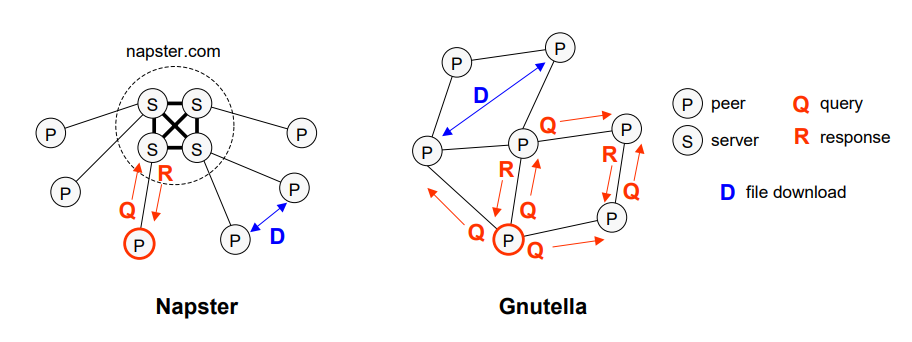
\includegraphics[width=.9\textwidth]{diagrams/napster-vs-gnutella.png}
    \caption{Napster vs Gnutella~\cite[Figure 1]{saroiu_measurement_2001}}
  \end{figure}
\end{center}

\subsubsection{Gnutella}

Peers using Gnutella will form an overlay network by having connections with sets of neighboring nodes, which are found using \textit{ping, pong} messages, where if a node receives a \textit{ping} message they send a \textit{originator} and forward the \textit{ping} to its neighbors. To download a file, a node will flood a message to its neighbors, who will check if they have it and return a message saying so. Regardless, the node will continue to flood through the overlay to find suitable peers.